% !TEX TS-program = XeLaTeX
% !TEX spellcheck = en-US
\documentclass[aspectratio=169]{beamer}

\usetheme{bi}

\title{Lecture 10:\\ Neural networks II}
\institute{GRA4160: Advanced Regression and Classification Analysis,\\
Ensemble Methods and Neural Networks}
\date{March 23rd 2023}
\author{Vegard H\o ghaug Larsen}

\begin{document}

\maketitle

\frame{
	\frametitle{Plan for today:}
	\begin{itemize}
		\item Multilayer neural networks
		\item Optimizers
		\item Weight initialization
		\item Dropout
		\item Convolutional neural networks
	\end{itemize}
}

%\frame{
%	\frametitle{The perceptron}
%}

\frame{
	\frametitle{Multi-layer neural networks}
	\begin{itemize}
		\item A multi-layer neural network is a neural network with more than one hidden layer
		\pause
		\item Modern neural networks typically have more than one hidden layer
		\pause
		%\item The hidden layers are used to learn more complex patterns in the data
		%\pause
		\item The number of hidden layers and the number of hidden units in each layer are hyperparameters that can be tuned
	\end{itemize}
}

\frame{
	\frametitle{Structure of a multilayer neural network}
	\begin{enumerate}
		\item \textbf{Input layer:} This is the first layer of the network, where input features are received. Each neuron in this layer corresponds to a feature from the input data
		\pause
		\item \textbf{Hidden layers:} These are the layers between the input and output layers. They are responsible for learning and extracting higher-level features from the input data. The number of hidden layers and the number of neurons in each hidden layer vary depending on the complexity of the problem
		\pause
		\item \textbf{Output layer:} This is the final layer of the network, responsible for producing the predictions or classification results. The number of neurons in this layer typically depends on the number of target classes or the desired output format
	\end{enumerate}
}

\frame{
	\frametitle{NN with two hidden layers and multiple outputs}
	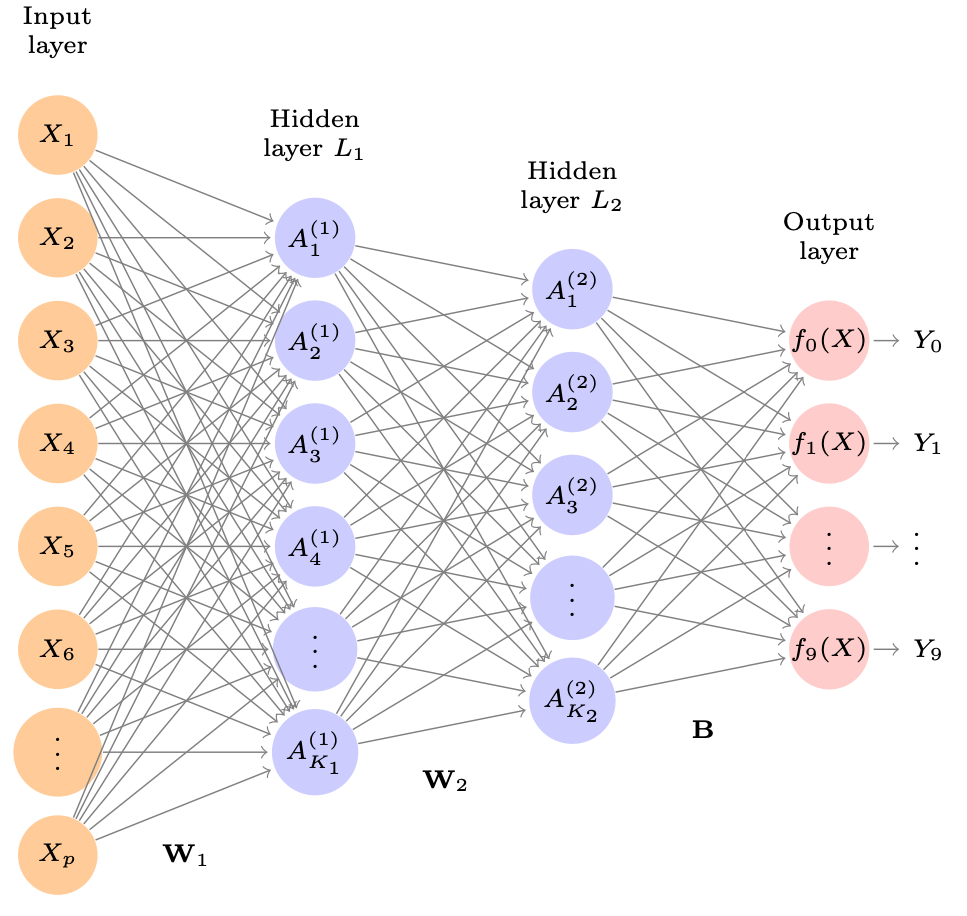
\includegraphics[scale=0.19]{figures/multilayer_NN.png}\\
	{\footnotesize Source: An Introduction to Statistical Learning with Applications in R, James, Witten, Hastie and Tibshirani, 2013}
}


\frame{
	\frametitle{Optimizers}
	\begin{enumerate}
		\item \textbf{Gradient descent}: The simplest algorithm that updates the weights by moving in the direction of the steepest decrease in the loss function, using the full dataset for each update
		\pause
		\item \textbf{Stochastic gradient descent}: A variant of Gradient Descent that updates the weights using a small random subset (mini-batch) of the training data which gives faster convergence
		%\item Mini-batch gradient descent
		\item \textbf{Momentum}: Adding momentum term to the weight updates, improving convergence by reducing oscillations and accelerating progress in directions with persistent gradients
		\pause
		%\item Nesterov momentum
		\item \textbf{Adagrad}: Adapts the learning rate for each weight based on the sum of squared gradients, allowing for different learning rates for different features
		\pause
		\item \textbf{RMSprop}: An improvement over AdaGrad that uses an exponential moving average of squared gradients instead of the cumulative sum, preventing the learning rate from becoming too small
		\pause
		\item \textbf{Adaptive Moment Estimation (Adam)}: A popular and efficient optimizer that combines ideas from AdaGrad and RMSProp.
	\end{enumerate}
}

\frame{
	\frametitle{Weight initialization}

	Weight initialization is the process of assigning initial values to the connection weights in a neural network before training begins
}

\frame{
	\frametitle{Importance of weight initialization}
	\begin{itemize}
		\item \textbf{Speed of convergence:} Proper weight initialization can help the network converge faster by starting the optimization process in a more favorable region of the weight space
		\pause
		\item \textbf{Avoiding symmetry breaking:} Problem that occurs when all neurons in a layer learn the same function
		\pause
		\item \textbf{Avoiding vanishing gradients:} Problem that occurs when the gradients of the loss function with respect to the weights become very small
		\pause
		\item \textbf{Avoiding exploding gradients:} Problem that occurs when the gradients of the loss function with respect to the weights become very large
		\pause
		\item \textbf{Escaping poor local minima:} Random weight initialization helps the network explore different regions of the weight space, reducing the likelihood of getting stuck in poor local minima
	\end{itemize}
}

\frame{
	\frametitle{Common weight initialization methods}
	\begin{itemize}
		\item \textbf{Zero initialization}: All weights are initialized to zero. This is a bad idea, because all neurons in a layer will learn the same function
		\pause
		\item \textbf{Random initialization}:  Assigning small random values to the weights is a simple and widely used technique. It can be done using various distributions, such as uniform or Gaussian
		\pause
		\item \textbf{Xavier initialization}: Weights are initialized randomly from a normal distribution with mean 0 and variance $\frac{1}{n_{in}}$, where $n_{in}$ is the number of input units to the layer
		\pause
		\item \textbf{He initialization}: Weights are initialized randomly from a normal distribution with mean 0 and variance $\frac{2}{n_{in}}$, where $n_{in}$ is the number of input units to the layer
	\end{itemize}
}

\frame{
	\frametitle{Dropout}
	\begin{itemize}
		\item \textbf{Dropout}: A regularization technique that randomly drops out (sets to zero) a fraction of the neurons in a layer during training. This forces the network to learn redundant representations, improving generalization
		\pause
		\item \textbf{Dropout rate}: The fraction of neurons that are dropped out during training. A dropout rate of 0.5 means that half of the neurons in a layer are dropped out
		\item Typically, dropout rates range from 0.1 to 0.5, with higher values leading to stronger regularization effects.
		%\pause
		%\item \textbf{Inference time}: During inference, the weights of the neurons that were dropped out during training are scaled up by a factor of $(1 - dropout\_rate)$ to compensate for the missing neurons
	\end{itemize}
}

\frame{
	\frametitle{Advantages of dropout}
	\begin{enumerate}
		\item \textbf{Regularization:} Acts as a regularizer by preventing the co-adaptation of neurons and encouraging the network to learn more robust and generalized features. This reduces the model's complexity and helps prevent overfitting.
		\pause
		\item \textbf{Implicit model averaging:} Can be seen as an ensemble method that trains multiple ``thinned´ networks with shared weights. These networks are combined, leading to an implicit model averaging that usually improves generalization.
		\pause
		\item \textbf{Speeding up training:} Can speed up training by reducing the number of neurons in a layer, reducing the number of parameters to be learned.
	\end{enumerate}
}

\frame{
	\frametitle{Introduction to Convolutional Neural Networks (CNNs)}
	CNNs are a type of neural network architecture specifically designed for processing grid-like data, such as images, where spatial relationships between inputs are important.
	\pause
	Key components of CNNs:
	\begin{itemize}
		\item \textbf{Convolutional layers:} Apply filters to the input, capturing local patterns within the data
		\item \textbf{Pooling layers:} Reduce spatial dimensions, increasing computational efficiency and promoting translational invariance
		\item  \textbf{Translational invariance:} Refers to the ability of the model to recognize and process patterns or features in the input data, regardless of their position within the image
		\item \textbf{Fully connected layers:} Combine features extracted by the convolutional and pooling layers to make predictions
	\end{itemize}
     \pause
CNNs have achieved state-of-the-art performance in various computer vision tasks, such as image classification, object detection, and semantic segmentation.
}

\frame{
	\frametitle{Convolutional layers}
	\begin{itemize}
		\item Apply a set of learnable filters (kernels) to the input
		\pause
		\item Each filter is a small matrix of weights that is convolved with the input to produce a feature map
		\pause
		\item Each filter slides (convolves) over the input, computing a dot product between the filter's weights and the input region (receptive field) it is covering
		\pause
		\item The result is a feature map that encodes local patterns and spatial relationships captured by the filter
		\pause
		\item Filters can learn to detect features such as edges, corners, and textures
	\end{itemize}
}

\frame{
	\frametitle{2D-convolutional layes}
	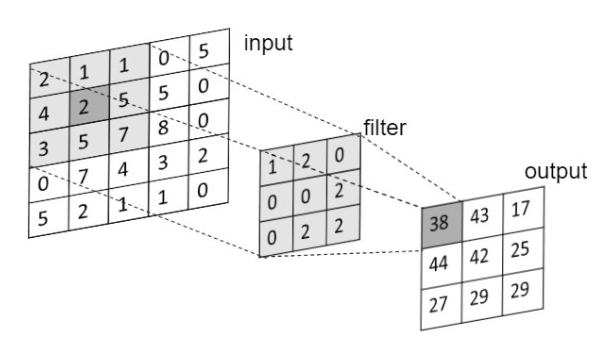
\includegraphics[scale=0.35]{figures/2d_convolution.png}\\
	{\footnotesize Source: Review: Deep Learning on 3D Point Clouds, Bello et al. 2020}

	\[38 = 2\cdot1 + 1\cdot2 + 1\cdot0 + 4\cdot0 + 2\cdot0 + 5\cdot2 + 3\cdot0 + 5\cdot2 + 7\cdot2  \]
}

\frame{
	\frametitle{Pooling layers}
	\begin{itemize}
		\item A pooling layer provides a way to condense a large image into a smaller summary image
		\pause
		\item Reduce the spatial dimensions of the feature maps, typically using operations such as max-pooling or average pooling
		\pause
		\item Max-pooling takes the maximum value within a pooling window, while average pooling takes the average value
		\pause
		\item Pooling promotes translational invariance and reduces computational complexity by decreasing the number of parameters
		\pause
		\item Pooling layers are often interleaved with convolutional layers in a CNN architecture
	\end{itemize}
}

\frame{
	\frametitle{Architecture of a deep CNN}
	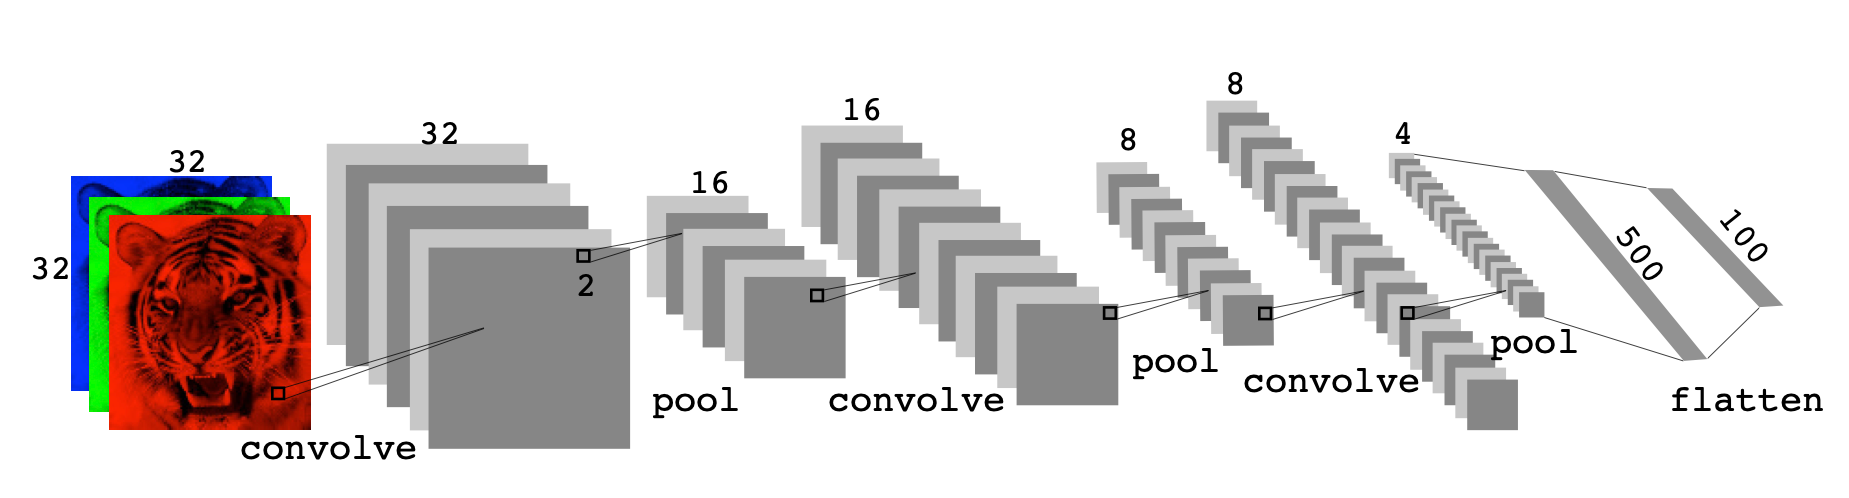
\includegraphics[scale=0.22]{figures/cnn.png}\\
	{\footnotesize Source: An Introduction to Statistical Learning with Applications in R, James, Witten, Hastie and Tibshirani, 2013}
}

\frame{
	\frametitle{Example of pooling}
	Consider a simple $2 \times 2$ input matrix for the pooling operation.
\[
A =
\begin{bmatrix}
a & b \\
c & d
\end{bmatrix}
\]
\pause
Max-pooling selects the maximum value from the input matrix.
\[
\text{max-pooling}(A) = \max(a, b, c, d)
\]
\pause
Average-pooling calculates the average value of the input matrix.
\[
\text{average-pooling}(A) = \frac{a + b + c + d}{4}
\]
}

\frame{
	\frametitle{Max-pooling and average-pooling}
\[ B =
\begin{bmatrix}
7 & 3 & 5 & 2 \\
2 & 8 & 4 & 7 \\
4 & 3 & 5 & 2 \\
3 & 2 & 4 & 5 \\
\end{bmatrix}
\]

\[ \text{max-pooling}(B) =\begin{bmatrix}
8 & 7 \\
4 & 5
\end{bmatrix},\;\;\;\; \text{average-pooling}(B) = \begin{bmatrix}
5 & 4.5 \\
3 & 4
\end{bmatrix} \]
}

%\frame{
%	\frametitle{Batch normalization}
%}

%\frame{
%	\frametitle{Padding}
%}

\end{document}

Introduction to Multilayer Neural Networks

Multilayer neural networks, also known as deep neural networks, consist of multiple layers of interconnected neurons arranged between the input and output layers. The layers between the input and output layers are called hidden layers. Each hidden layer can be seen as a transformation or feature extraction process that helps the network learn complex patterns from the input data.

Structure of a Multilayer Neural Network

Input layer: This is the first layer of the network, where input features are received. Each neuron in this layer corresponds to a feature from the input data.
Hidden layers: These are the layers between the input and output layers. They are responsible for learning and extracting higher-level features from the input data. The number of hidden layers and the number of neurons in each hidden layer vary depending on the complexity of the problem.
Output layer: This is the final layer of the network, responsible for producing the predictions or classification results. The number of neurons in this layer typically depends on the number of target classes or the desired output format.
Activation Functions

Activation functions play a critical role in multilayer neural networks. They introduce nonlinearity into the network, allowing it to learn complex and nonlinear patterns from the data. Common activation functions include the sigmoid, hyperbolic tangent (tanh), and rectified linear unit (ReLU).

Advantages of Multilayer Neural Networks

Representation learning: Multilayer neural networks can automatically learn useful representations and features from raw data, reducing the need for manual feature engineering.
Nonlinear modeling: Due to the presence of activation functions, these networks can model complex, nonlinear relationships between inputs and outputs.
Universality: Multilayer neural networks are universal function approximators, meaning they can approximate any continuous function, given a sufficient number of neurons and layers.
Scalability: Deep learning frameworks make it relatively easy to scale and train large neural networks on massive datasets using parallel and distributed computing.
Challenges

While multilayer neural networks offer numerous benefits, they also come with challenges, including:

Training complexity: Deeper networks with many layers require more computational resources and time to train.
Overfitting: Networks with a large number of parameters are prone to overfitting, especially when dealing with limited or noisy training data.
Interpretability: Understanding the internal workings of a multilayer neural network can be challenging, making it difficult to explain the reasoning behind their predictions.
Vanishing/exploding gradients: During training, gradients can become very small (vanish) or very large (explode), leading to slow convergence or instability.
In summary, multilayer neural networks provide a powerful tool for tackling complex machine learning tasks. By combining multiple layers of neurons with nonlinear activation functions, these networks can learn hierarchical representations of input data and model intricate relationships. However, they also come with challenges that researchers and practitioners must address to ensure successful implementation.